\section{Moment Realizability and Closures for Fermion}
\label{sec:realizability}

Our goal is to design a numerical method for solving the system of equations given by Eq.~\eqref{eq:momentEquations}, which approximates Eq.~\eqref{eq:boltzmann}.  
To this end, we want to obtain solutions that preserve features of the original problem. 

Since we only consider the angular dependence of the distribution function in this section, we simplify the notation by suppressing the $\vect{z}$ and $t$ dependence, and write $f(\omegaNu,\vect{z},t)=f(\omegaNu)$.  

\subsection{Moment Realizability}

\begin{define}
  The moments $\vect{\cM}=\big(\cJ,\vect{\cH}\big)^{T}$ are realizable if they are consistent with a distribution function satisfying $0\le f(\omegaNu) \le 1$.
\end{define}

We begin by stating the bounds on the moments by restating results from Theorem~7.1 in \cite{banachLarecki_2017} in the following Lemma.  
\begin{lemma}
  Let the distribution function be bounded by $0\le f(\omegaNu) \le1$ for all $\omegaNu\in\bbS^{2}$.  
  Then $0\le\cJ\le1$ and $\big(1-\cJ\big)\,\cJ-|\vect{\cH}|\ge0$. 
  \label{lem: MomentRealizable} 
\end{lemma}
\begin{proof}
  First, let $\mu=\cos\thetaNu$ and write
  \begin{equation}
    \cJ=\f{1}{2}\int_{\bbS^{1}}\mathfrak{f}(\mu)\,d\mu,
    \quad\text{where}\quad
    \mathfrak{f}(\mu)=\f{1}{2\pi}\int_{0}^{2\pi}f(\mu,\phiNu)\,d\phiNu.  
  \end{equation}  
  Since $f(\omegaNu)\in[0,1]$, we have $\mathfrak{f}(\mu)\in[0,1]$, which implies $\cJ\in[0,1]$.  
  Next we need to show that $|\vect{\cH}|\le(1-\cJ)\,\cJ$.  
  Let $\widehat{\vect{n}}\in\bbR^{3}$ (independent of $\omegaNu$) be an arbitrary unit vector, and write
  \begin{equation}
    \widehat{\vect{n}}\cdot\vect{\cH}
    =\int_{\bbS^{1}}\mathfrak{f}(\mu)\,\mu\,d\mu,
    \label{eq:NdotH}
  \end{equation}
  where we have aligned the polar axis of the spherical momentum space coordinate system with $\widehat{\vect{n}}$; i.e., $\widehat{\vect{n}}\cdot\vect{\ell}(\omega)=\mu$.  
  First, following \cite{banachLarecki_2017}, we can write the integral on the right-hand side of Eq.~\eqref{eq:NdotH} as
  \begin{equation*}
    (1-\cJ)\cJ - \f{1}{2}\int_{-1}^{1-2\cJ}(1-2\cJ-\mu)\,\mathfrak{f}(\mu)\,d\mu
    -\f{1}{2}\int_{1-2\cJ}^{1}(2\cJ-1+\mu)\,[1-\mathfrak{f}(\mu)]\,d\mu.  
  \end{equation*}
  Since $\mathfrak{f}\in[0,1]$, $(1-2\cJ-\mu)$ is nonnegative on the interval $\mu\in[-1,1-2\cJ]$, and $(2\cJ-1+\mu)$ is nonnegative on the interval $\mu\in[1-2\cJ,1]$, we have $\widehat{\vect{n}}\cdot\vect{\cH}\le(1-\cJ)\,\cJ$.  
  In a similar manner, we can also write the integral on the right-hand side of Eq.~\eqref{eq:NdotH} as
  \begin{equation*}
    -(1-\cJ)\cJ-\f{1}{2}\int_{-1}^{2\cJ-1}(1-2\cJ+\mu)\,[1-\mathfrak{f}(\mu)]\,d\mu
    -\f{1}{2}\int_{2\cJ-1}^{1}(2\cJ-1-\mu)\,\mathfrak{f}(\mu)\,d\mu.  
  \end{equation*}
  Then, since $\mathfrak{f}\in[0,1]$, $(1-2\cJ+\mu)$ is nonpositive on the interval $\mu\in[-1,2\cJ-1]$, and $(2\cJ-1-\mu)$ is nonpositive on the interval $\mu\in[2\cJ-1,1]$, we have $\widehat{\vect{n}}\cdot\vect{\cH}\ge-(1-\cJ)\,\cJ$.  
  We therefore have $-(1-\cJ)\,\cJ\le\widehat{\vect{n}}\cdot\vect{\cH}\le(1-\cJ)\,\cJ$.  
  Since this holds for any unit vector $\widehat{\vect{n}}\in\bbR^{3}$, we must have $|\vect{\cH}|\le(1-\cJ)\,\cJ$.  
\end{proof}

We now define the realizable set $\cR$
\begin{equation}
  \cR:=\big\{\,\vect{\cM}=\big(\cJ,\vect{\cH}\big)^{T}~|~\cJ\in[0,1]~\text{and}~\gamma(\vect{\cM})\equiv(1-\cJ)\cJ-|\vect{\cH}|\ge0\,\big\}
  \label{eq:realizableSet}
\end{equation}

\begin{lemma}
  The set $\cR$, defined in Eq.~\eqref{eq:realizableSet}, is convex.  
\end{lemma}
\begin{proof}
  A convex set $Q$ is a set has the following property: 
  \begin{equation*}
  \theta a + (1-\theta)b \in Q,~\text{for}~\forall a, b \in Q~\text{and}~0\leq\,\theta\,\leq1. 
  \end{equation*} 
  Let $\vect{\cM}_{a}=\big(\cJ_{a},\vect{\cH}_{a}\big)^{T}$ and $\vect{\cM}_{b}=\big(\cJ_{b},\vect{\cH}_{b}\big)^{T}$ to be two arbitrary elements of $\cR$.
  If $\cR$ is convex, we will have $\vect{\cM}_{ab} = \big(\cJ_{ab},\vect{\cH}_{ab}\big)^{T} = \theta \vect{\cM}_{a} + (1-\theta)\vect{\cM}_{b}$ in $\cR$ with $0\leq\theta\leq1$.
  The first component of $\vect{\cM}_{ab}$ is
  \begin{equation*}
  \cJ_{ab} = \theta \cJ_{a} + (1-\theta)\cJ_{b}.
  \end{equation*}
  Since $\theta$, $\cJ_{a}$, $1-\theta$ and $\cJ_{b}$ are all nonnegative, $\cJ_{ab}$ is also nonnegative.
  Meanwhile, since $\cJ_{a}\leq1$ and $\cJ_{b}\leq1$, $\cJ_{ab}\leq1$.
  That's $\cJ_{ab} \in [0,1]$.
  Since the second derivative of $\gamma(\vect{\cM})$ is $-2$ which is always negative, $\gamma(\vect{\cM})$ is a concave function.
  Using Jensen's inequality, we have
  \begin{equation*}
  \gamma(\vect{\cM_{ab}}) \geq \theta\gamma(\vect{\cM_{a}}) + (1-\theta)\gamma(\vect{\cM_{b}}) \ge0.
  \end{equation*}
\end{proof}

The Fig.~\ref{fig:RealizableSetFermionic} illustrates how the convex realizable set $\cR$ looks like in $|\vect{\cH}| - \cJ$ coordinates.
Total 1000,000 distribution functions having form $\mathfrak{f}(\mu;a,b) = \dfrac{1}{e^{a+b\mu}+1}$ were evaluated.
The parameters, $a$ and $b$, were chosen from $[-100,100]$ independently.
The variable $\mu$ ranges from $-1$ to $1$ with $d\mu=\f{1}{128}$.
And the integrals in angular moment expressions are calculated using Trapezoid rule.
\begin{figure}
\centering
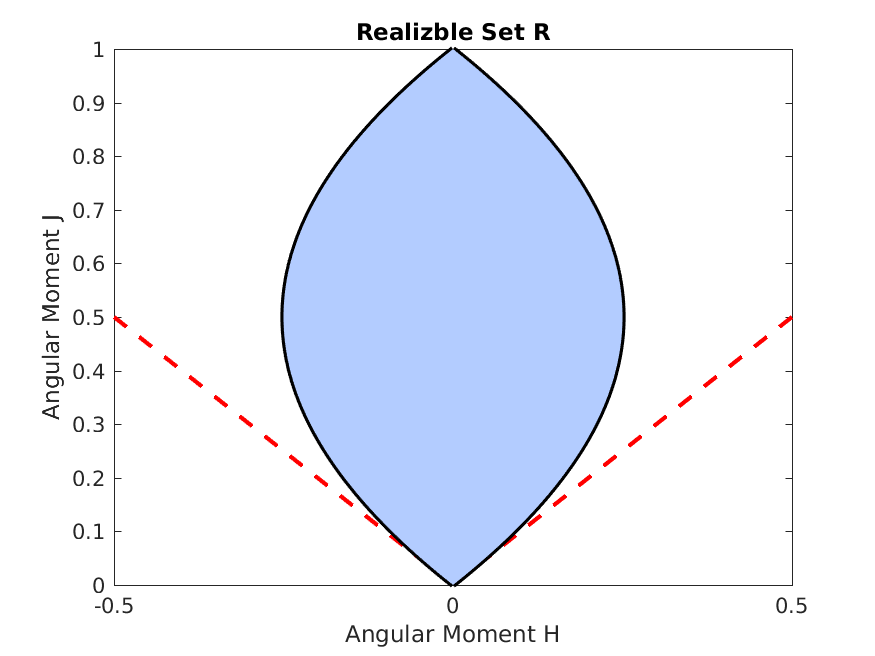
\includegraphics[width=1.0\linewidth]{figures/RealizableSetFermionic}
\caption[Numerical plot of the convex realizable set $\cR$.]{
A numerical plot of the convex realizable set $\cR$.
The black line are the boundary given by $\gamma(\vect{\cM}) = 0$. 
The red line are the boundary given by $|\vect{\cH}| = \cJ$.
Every light-blue dot represents a sample whose distribution function $\mathfrak{f}(\mu)$ is an arbitrary Fermi-Dirac function and its angular moments were given by integrals using Trapezoid rule.
Total 1000,000 $\mathfrak{f}(\mu)$ were sampled for making this plot.}
\label{fig:RealizableSetFermionic}
\end{figure}

\begin{lemma}
  Let $\big\{\cJ_{a},\vect{\cH}_{a},\vect{\cK}_{a}\big\}$ be defined as in Eq.~\eqref{eq:angularMoments} with distribution function $f_{a}\in[0,1]$.  
  Similarly, $\big\{\cJ_{b},\vect{\cH}_{b},\vect{\cK}_{b}\big\}$ be moments of a distribution function $f_{b}\in[0,1]$.  
  Let $\Phi^{\pm}(\vect{\cM})=\f{1}{2}\big(\vect{\cM}\pm\widehat{\vect{e}}\cdot\vect{\cF}(\vect{\cM})\big)$, where $\widehat{\vect{e}}\in\bbR^{3}$ is an arbitrary unit vector.  
  Then
  \begin{equation}
    \Phi^{+}(\vect{\cM}_{a})+\Phi^{-}(\vect{\cM}_{b})\in\cR.
  \end{equation}
\end{lemma}
\begin{proof}
  The first component of $\Phi^{+}(\vect{\cM}_{a})+\Phi^{-}(\vect{\cM}_{b})$ is
  \begin{equation*} 
    \f{1}{2}\big(\vect{\cJ_{a}} + \widehat{\vect{e}}\cdot\vect{\cF}(\vect{\cJ_{a}})+\vect{\cJ_{b}} - \widehat{\vect{e}}\cdot\vect{\cF}(\vect{\cJ_{b}})\big) = \f{1}{2}\big(\vect{\cJ_{a}} + \widehat{\vect{e}}\cdot\vect{\cH_{a}}+\vect{\cJ_{b}} - \widehat{\vect{e}}\cdot\vect{\cH_{b}}\big).
  \end{equation*}
  Using the same treatment we made in proof of Lemma~\ref{lem: MomentRealizable}, we can rewrite the first component as
  \begin{align*}
  &\f{1}{2} \left\lbrace \f{1}{2}\int_{\bbS^{1}}\left[ \mathfrak{f}_{a}(\mu)\,(1+\mu) + \mathfrak{f}_{b}(\mu)\,(1-\mu)\right] \,d\mu \right\rbrace \\
  \equiv  &\f{1}{2}\int_{\bbS^{1}} \mathfrak{f}_{ab}(\mu)\,d\mu \\
  \text{where}&~\mathfrak{f}_{ab}(\mu) \equiv \f{1}{2}\left[ \mathfrak{f}_{a}(\mu)\,(1+\mu) + \mathfrak{f}_{b}(\mu)\,(1-\mu)\right].
  \end{align*}
  We know that $\f{1}{2}(1\pm\mu)\in[0,1]$, $\mathfrak{f}_{a}(\mu)\in[0,1]$ and $\mathfrak{f}_{b}(\mu)\in[0,1]$, therefore $\mathfrak{f}_{ab}(\mu)\in[0,1]$ and the first component is also in $[0,1]$.
  The second component
  \begin{equation*} 
    \f{1}{2}\big(\vect{\cH_{a}} + \widehat{\vect{e}}\cdot\vect{\cF}(\vect{\cH_{a}})+\vect{\cH_{b}} - \widehat{\vect{e}}\cdot\vect{\cF}(\vect{\cH_{b}})\big) = \f{1}{2}\big(\vect{\cH_{a}} + \widehat{\vect{e}}\cdot\vect{\cK_{a}}+\vect{\cH_{b}} - \widehat{\vect{e}}\cdot\vect{\cK_{b}}\big)
  \end{equation*}  
  has three subcomponents and each of them can also be rewritten as
  \begin{align*}
    \f{1}{2} \left\lbrace \f{1}{2}\int_{\bbS^{1}}\left[ \mathfrak{f}_{a}(\mu)\,(1+\mu) + \mathfrak{f}_{b}(\mu)\,(1-\mu)\right]\mu \,d\mu \right\rbrace
     \equiv  &\f{1}{2}\int_{\bbS^{1}} \mathfrak{f}_{ab}(\mu)\,\mu d\mu. 
  \end{align*}
  Therefore, using Lemma~\ref{lem: MomentRealizable} we know that $\Phi^{+}(\vect{\cM}_{a})+\Phi^{-}(\vect{\cM}_{b})\in\cR$.
\end{proof}

\subsection{Moment Closures}

Flux factor $h=|\vect{\cH}|/\cJ$
\begin{equation}
  \chi(\cJ,h)=\f{1}{3}+\f{2\,(1-\cJ)\,(1-2\cJ)}{3}\,\Theta\Big(\f{h}{1-\cJ}\Big)
\end{equation}

\subsubsection{Maximum Entropy Closure}
Basic principles
Chernohorsky \& Bludman \cite{cernohorskyBludman_1994}
\begin{equation}
  \Theta_{\mbox{\tiny ME}}^{\mbox{\tiny CB}}(x)
  =x^{2}\,\big(\,3-x+3\,x^{2}\,\big)
\end{equation}
Banach \& Larecki
\begin{equation}
  \Theta_{\mbox{\tiny ME}}^{\mbox{\tiny BL}}(x)
  =\f{1}{8}\,\big(\,9\,x^{2}-5+\sqrt{33\,x^{4}-42\,x^{2}+25}\,\big)
\end{equation}

\subsubsection{Kershaw Closure}
Basic principles
Banach \& Larecki \cite{banachLarecki_2017}
\begin{equation}
  \Theta_{\mbox{\tiny K}}^{\mbox{\tiny BL}}(x)=x^{2}
\end{equation}

\subsubsection{Low Occupancy Limit}